
\documentclass[14pt]{extbook}
%General Packages
\usepackage{multicol, enumerate, enumitem, hyperref, color, soul, setspace, parskip, fancyhdr}

%Math Packages
\usepackage{amssymb, amsthm, amsmath, bbm, latexsym, units, mathtools}

%All math in Display Style
\everymath{\displaystyle}

% Packages with additional options
%\usepackage[T1]{fontenc}
\usepackage[headsep=0.5cm,headheight=12pt, left=1 in,right= 1 in,top= 1 in,bottom= 1 in]{geometry}
\usepackage[usenames,dvipsnames]{xcolor}

% SageTeX
\usepackage{sagetex}

% Package to use the command below to create lines between items
\usepackage{dashrule}
\newcommand{\litem}[1]{\item#1\hspace*{-1cm}\rule{\textwidth}{0.4pt}}

\pagestyle{fancy}
\lhead{Module\,11M\,-\,Modeling\,with\,Log\,and\,Exp\,Functions}
\chead{}
\rhead{Progress Exam 6}
\lfoot{Summer\,C\,2020}
\cfoot{}
\rfoot{Version A}

\begin{document}
\pagestyle{fancy}

\begin{sagesilent}
load("../Code/pythonImports.sage")
load("../Code/intervalMaskingMethod.sage")
load("../Code/keyGeneration.sage")
load("../Code/commonlyUsedFunctions.sage")
keyFileName = "Module11M"
version = "A"
\end{sagesilent}

\begin{enumerate}
%\setcounter{enumi}{50}


  \begin{sagesilent}
  moduleNumber="11M"
  problemNumber=51
  load("../Code/11modelingLogExp/identifyModelGraph11.sage")
  \end{sagesilent}

  \litem{ \sage{displayStem}

   \begin{center}
       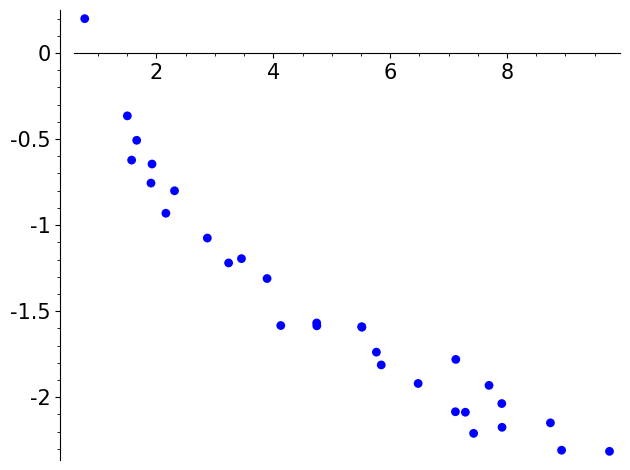
\includegraphics[width=0.5\textwidth]{../Figures/identifyModelGraph11A.png}
   \end{center}

  	\begin{enumerate}[label=\Alph*.]
    \item \( \sage{choices[0]} \)
    \item \( \sage{choices[1]} \)
    \item \( \sage{choices[2]} \)
    \item \( \sage{choices[3]} \)
    \item \( \sage{choices[4]} \)
  	\end{enumerate}
  }

\begin{sagesilent}
moduleNumber="11M"
problemNumber=52
load("../Code/11modelingLogExp/constructTemperatureModel.sage")
\end{sagesilent}

  \litem{ \sage{displayStem}

   \begin{center}
      \textit{ \sage{displayProblem} }
   \end{center}

  	\begin{enumerate}[label=\Alph*.]
    \item \( \sage{choices[0]} \)
    \item \( \sage{choices[1]} \)
    \item \( \sage{choices[2]} \)
    \item \( \sage{choices[3]} \)
    \item \( \sage{choices[4]} \)
  	\end{enumerate}
  }

  \begin{sagesilent}
  moduleNumber="11M"
  problemNumber=53
  load("../Code/11modelingLogExp/identifyModelPopulation.sage")
  \end{sagesilent}

  \litem{ \sage{displayStem}

  \begin{tabular}{c|c|c|c|c|c|c|c|c|c}
    \textbf{Year} & 1 & 2 & 3 & 4 & 5 & 6 & 7 & 8 & 9 \tabularnewline
    \hline
    \textbf{Pop.} & \sage{populations[0]} & \sage{populations[1]} & \sage{populations[2]} & \sage{populations[3]} & \sage{populations[4]} & \sage{populations[5]} & \sage{populations[6]} & \sage{populations[7]} & \sage{populations[8]}
  \end{tabular}

  	\begin{enumerate}[label=\Alph*.]
    \item \( \sage{choices[0]} \)
    \item \( \sage{choices[1]} \)
    \item \( \sage{choices[2]} \)
    \item \( \sage{choices[3]} \)
    \item \( \sage{choices[4]} \)
  	\end{enumerate}
  }

\begin{sagesilent}
moduleNumber="11M"
problemNumber=54
load("../Code/11modelingLogExp/constructHalfLifeModel.sage")
\end{sagesilent}

  \litem{ \sage{displayStem}

   \begin{center}
      \textit{ \sage{displayProblem} }
   \end{center}

  	\begin{enumerate}[label=\Alph*.]
    \item \( \sage{choices[0]} \)
    \item \( \sage{choices[1]} \)
    \item \( \sage{choices[2]} \)
    \item \( \sage{choices[3]} \)
    \item \( \sage{choices[4]} \)
  	\end{enumerate}
  }

\begin{sagesilent}
moduleNumber="11M"
problemNumber=55
load("../Code/11modelingLogExp/constructBacteriaGrowth.sage")
\end{sagesilent}

  \litem{ \sage{displayStem}

   \begin{center}
      \textit{ \sage{displayProblem} }
   \end{center}

  	\begin{enumerate}[label=\Alph*.]
    \item \( \sage{choices[0]} \)
    \item \( \sage{choices[1]} \)
    \item \( \sage{choices[2]} \)
    \item \( \sage{choices[3]} \)
    \item \( \sage{choices[4]} \)
  	\end{enumerate}
  }

\end{enumerate}

\end{document}

